\documentclass[a4paper,11pt]{article}
\usepackage[utf8]{inputenc}
\usepackage[russian]{babel}
\usepackage[T1]{fontenc}
\usepackage{amssymb,amsmath,clrscode,graphicx,indentfirst}

\author{Иван Веселов}
\title{Курс kiev-clrs -- Лекция 11. Расширение структур данных. Деревья отрезков.}
\date{2009 г.}

\begin{document}

\maketitle
\tableofcontents
\newpage

\setlength{\parskip}{1ex plus 0.5ex minus 0.2ex}

\section{План лекции}
\begin{itemize}
\item Динамические порядковые статистики
\item Методология расширения структур данных
\item Деревья отрезков
\end{itemize}

\section{Введение}

Сегодня мы познакомимся с расширением структур данных. Это весьма
распространённый и общепринятый подход: в процессе решения задачи мы обычно не создаём
новые структуры данных ``с нуля'', а скорее дополняем или расширяем уже
существующие структуры в своих целях. Это и называется расширение структур
данных.

\section{Динамические порядковые статистики}

Мы уже знакомы с порядковыми статистиками, медианами и т.д. и находили их в
массиве. Теперь предположим, что нам нужно найти порядковые статистики в
динамическом множестве, в которое мы можем добавлять и удалять элементы.

Введём следующие дополнительные операции для нашего множества:

OS-Select(i, S) -- возвращает $i$-й по порядку элементы ($i$-й наименьший
элемент)

OS-Rank(x, S) -- возвращает ранг $x \in S$ если множество $S$ отсортировано

Идея: использовать для представления множества красно-чёрное дерево и хранить в
его узлах размер поддеревьев этого узла.

\begin{center}
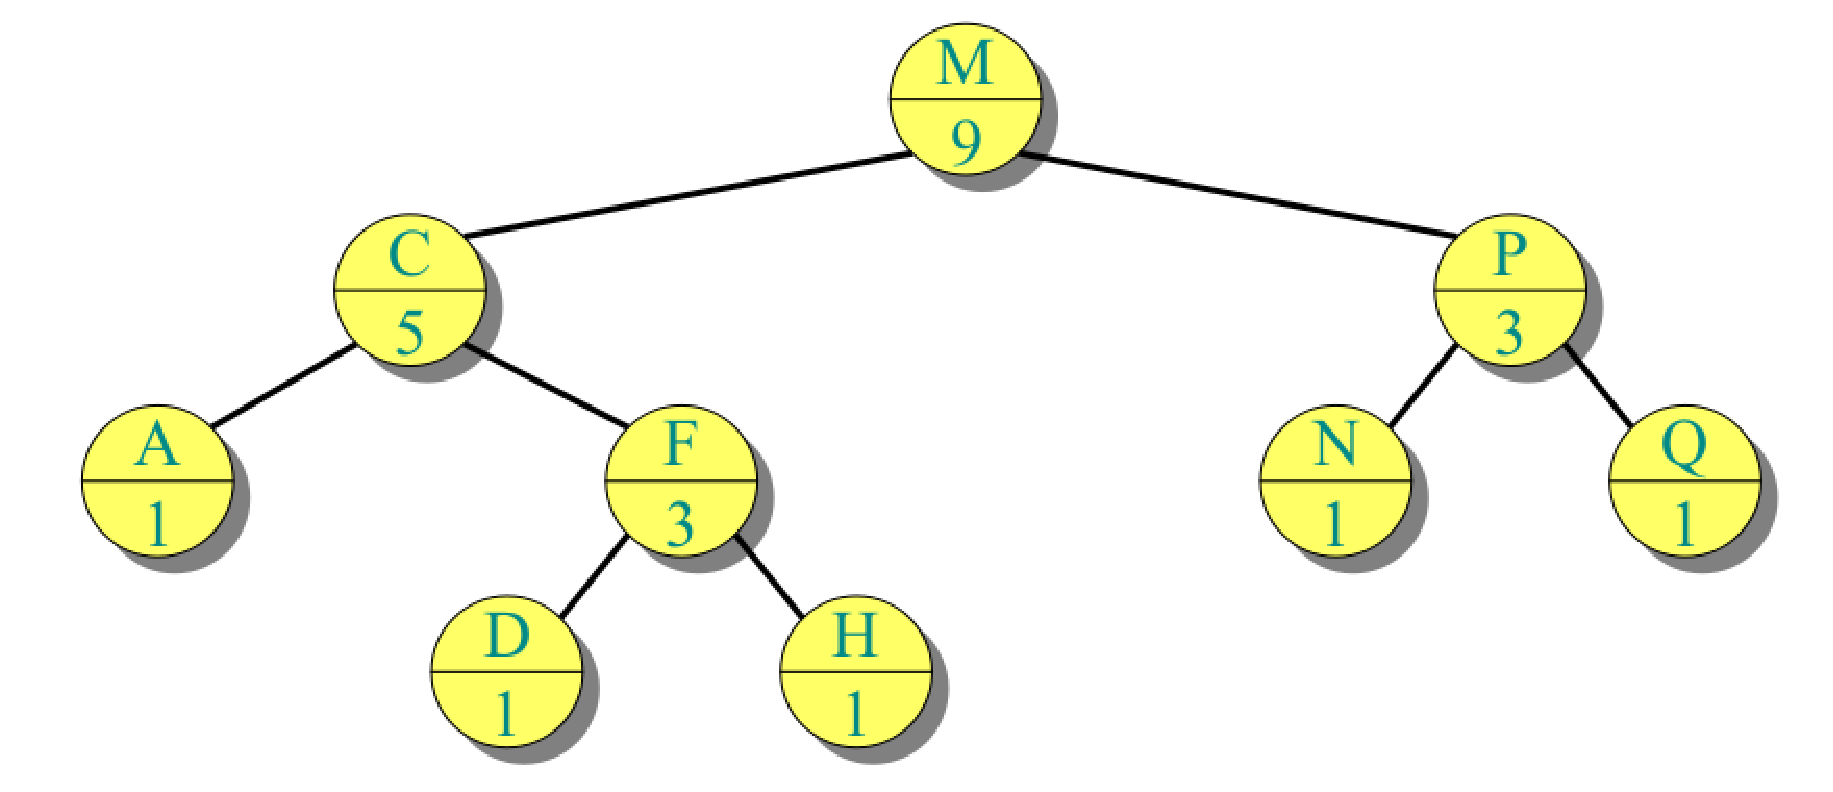
\includegraphics[width=5in]{lecture11/tree1.eps}
\end{center}

$$
size[x] = size[left[x]] + size[right[x]] + 1
$$

Храним в нодах два значения: ключ и размер поддеревьев.

(Предложить раскрасить дерево самостоятельно!)

Есть небольшая проблема с определением размера листьев дерева, т.к. у них левый
и правый ребёнок -- налл. Размер налла, очевидно, ноль, но это может вызвать
ошибку. И для того чтобы не загромождать алгоритм проверками на налл, часто
используют так называемый sentinel, фиктивная нода, такая что size[sentinel] = 0. И
вместо того чтобы хранить налл, листья указывают на эту фиктивную ноду.

\begin{codebox}
\Procname{$\proc{OS\_Select}(x, i)$} 
\li $k \gets size[left[x]] + 1$ \Comment $k = rank[x]$
\li \If $i = k$
\li \Then \Return x
    \End
\li \If $i < k$
\li \Then \Return $\proc{OS\_Select}(left[x], i)$
\li \Else \Return $\proc{OS\_Select}(right[x], i - k)$
    \End
\end{codebox}

Пример: нахождение пятого по порядку элемента, т.e. $\proc{OS\_Select}(root, 5)$:

\begin{center}
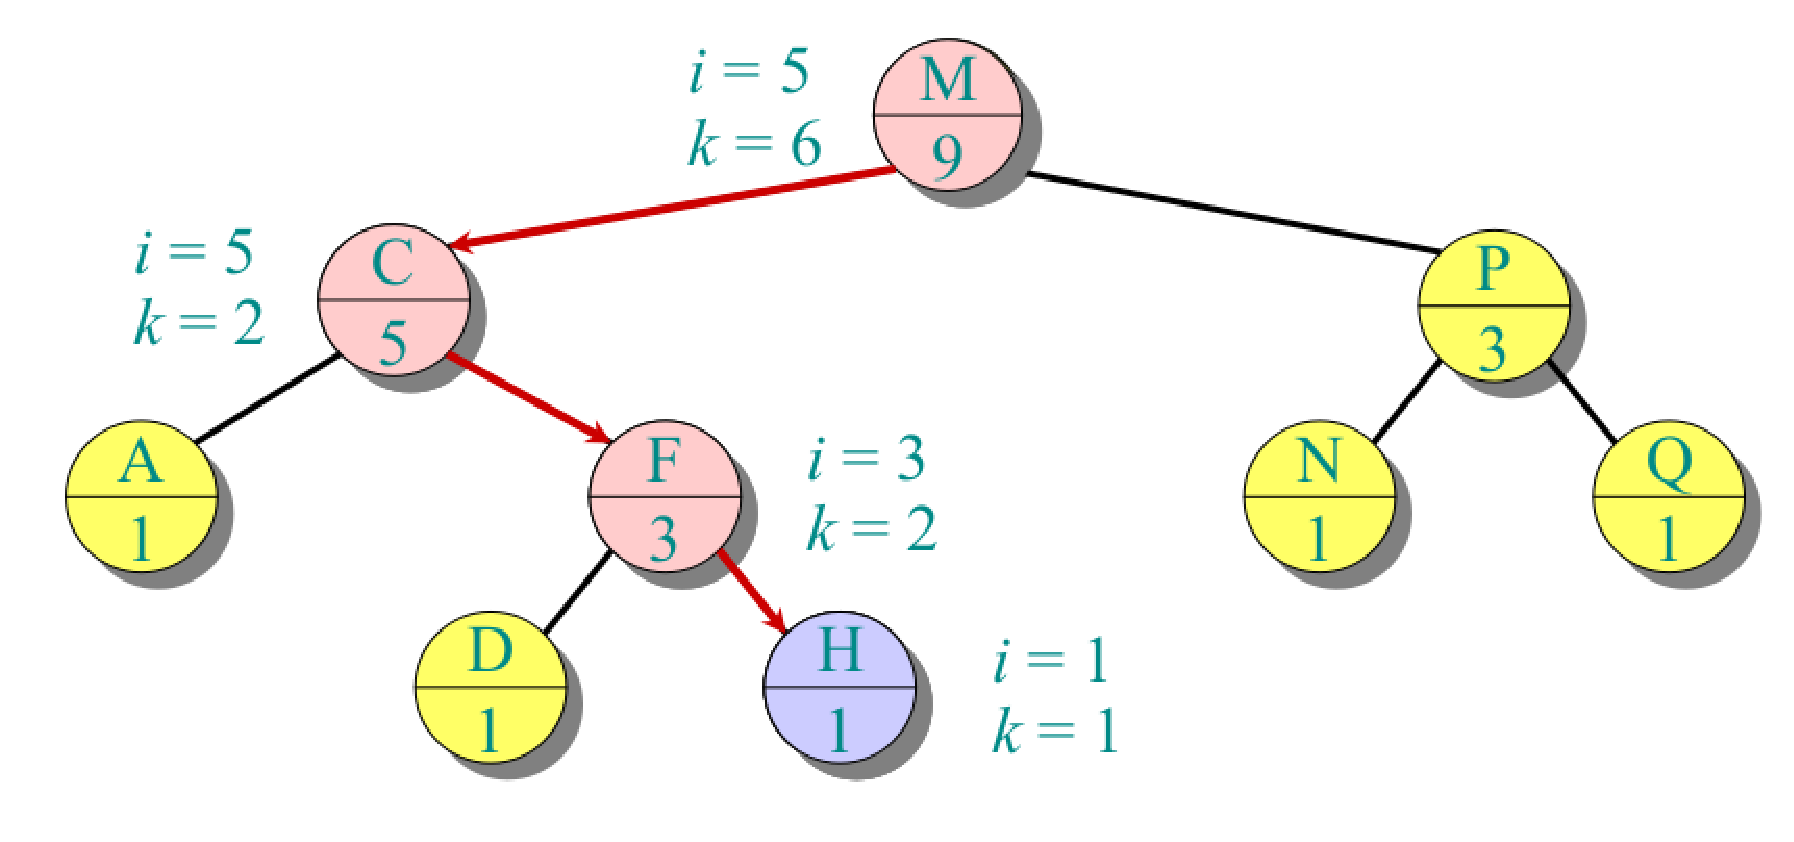
\includegraphics[width=5in]{lecture11/tree2.eps}
\end{center}

Анализ: $\proc{OS\_Select}$ выполняется за $O(\lg n)$ операций, поскольку это
красно-чёрное дерево.

Вопрос: почему бы не хранить сами ранги в дереве?

Ответ: неудобно поддерживать дерево. При вставке элемента в начало, придётся
обновить все ранги. В случае же хранение размеров поддеревьев -- только $\log n$
(вверх от элемента до корня дерева).

При расширении структуры данных важно понимать, что не только новые, добавленные
операции должны работать быстро, но при этом и старые, уже существовашие в
базовой структуре операции не должны стать медленнее. Нужно сохранять их
свойства, корректность и производительность.

Модифицирующие операции: вставка и удаление.

Стратегия сохранения свойств при вставке: пересчитывать размеры поддеревьев
нескольких нод в процессе вставки.

Пример вставки элемента К:
\begin{center}
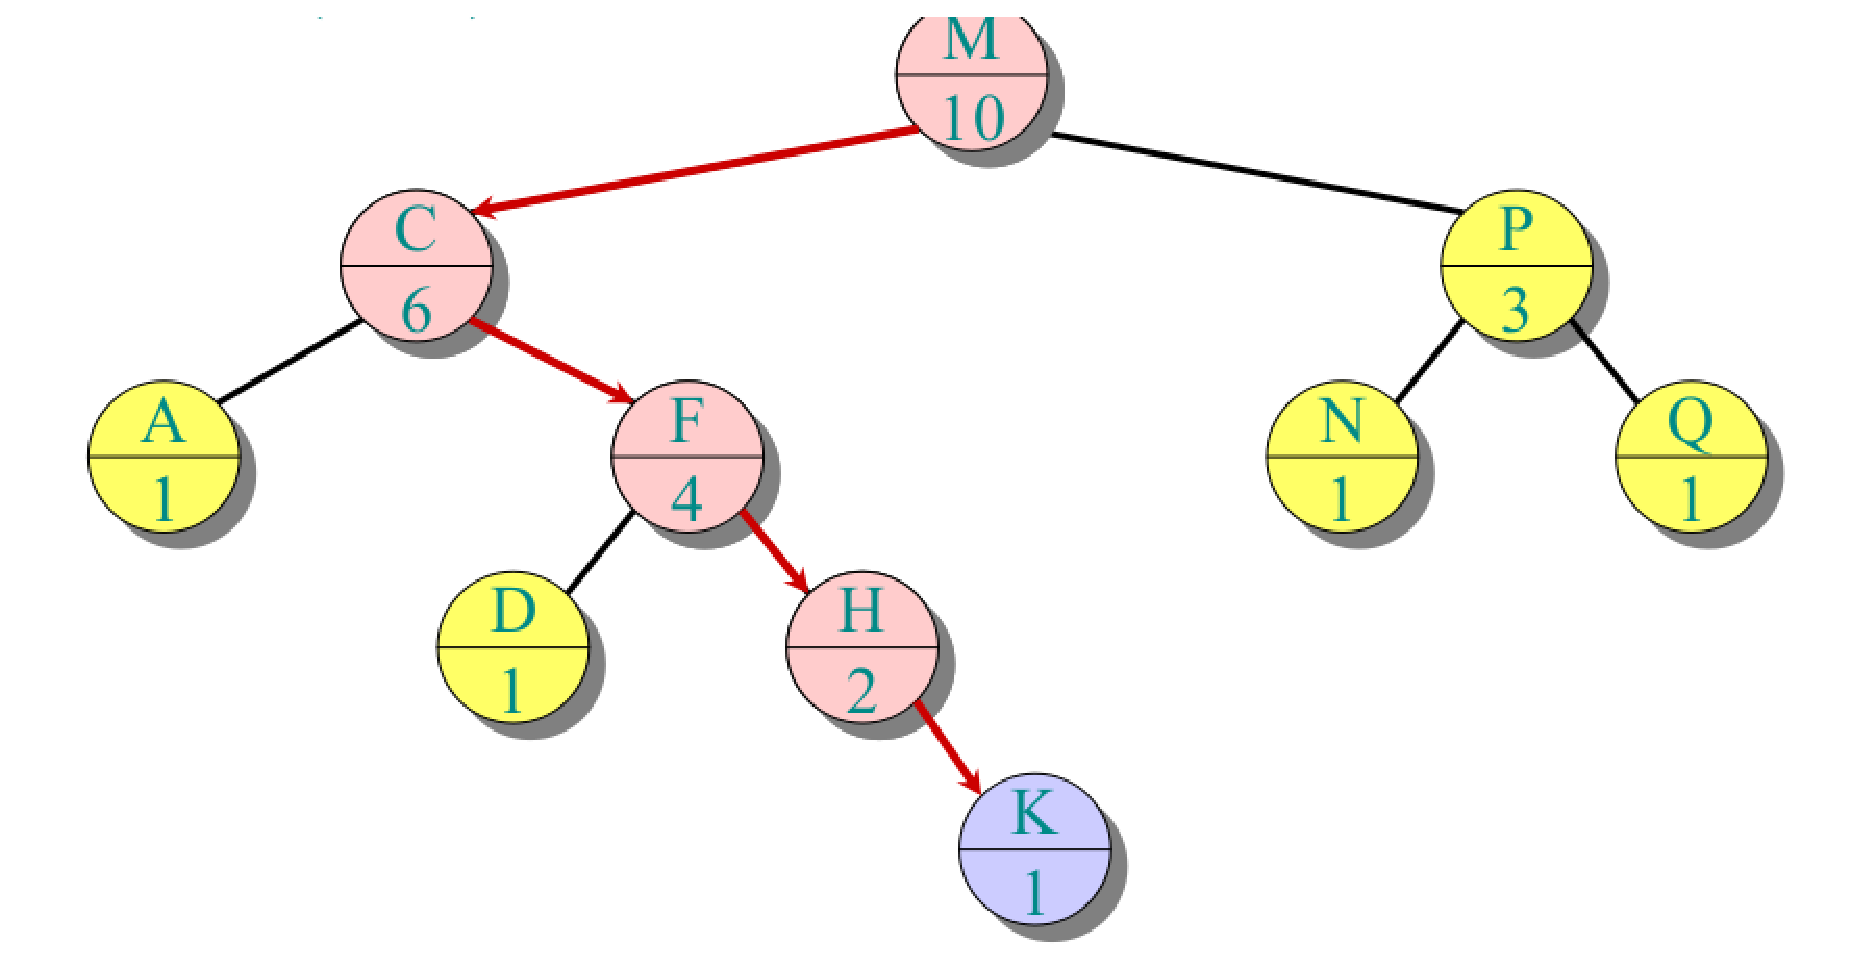
\includegraphics[width=5in]{lecture11/tree3.eps}
\end{center}

Кроме вставки элемента как в обычное бинарное дерево мы должны провести и
ребалансировку дерева.

Ребалансирующие операции:
\begin{itemize}
\item изменение цветов узлов -- не структурное изменение дерева, потому не
  требуется менять значения размера поддерева
\item поворот -- меняется структура, значит нужно пересчитывать и размер
  поддерева. Мы можем сделать это за $O(1)$ шагов, поскольку может быть только
  два поворота за один шаг и в процессе пересчёта мы пересчитываем размеры
  поддервьев только у одной ноды на основе её детей.
\end{itemize}

Повороты и пересчёты:
\begin{center}
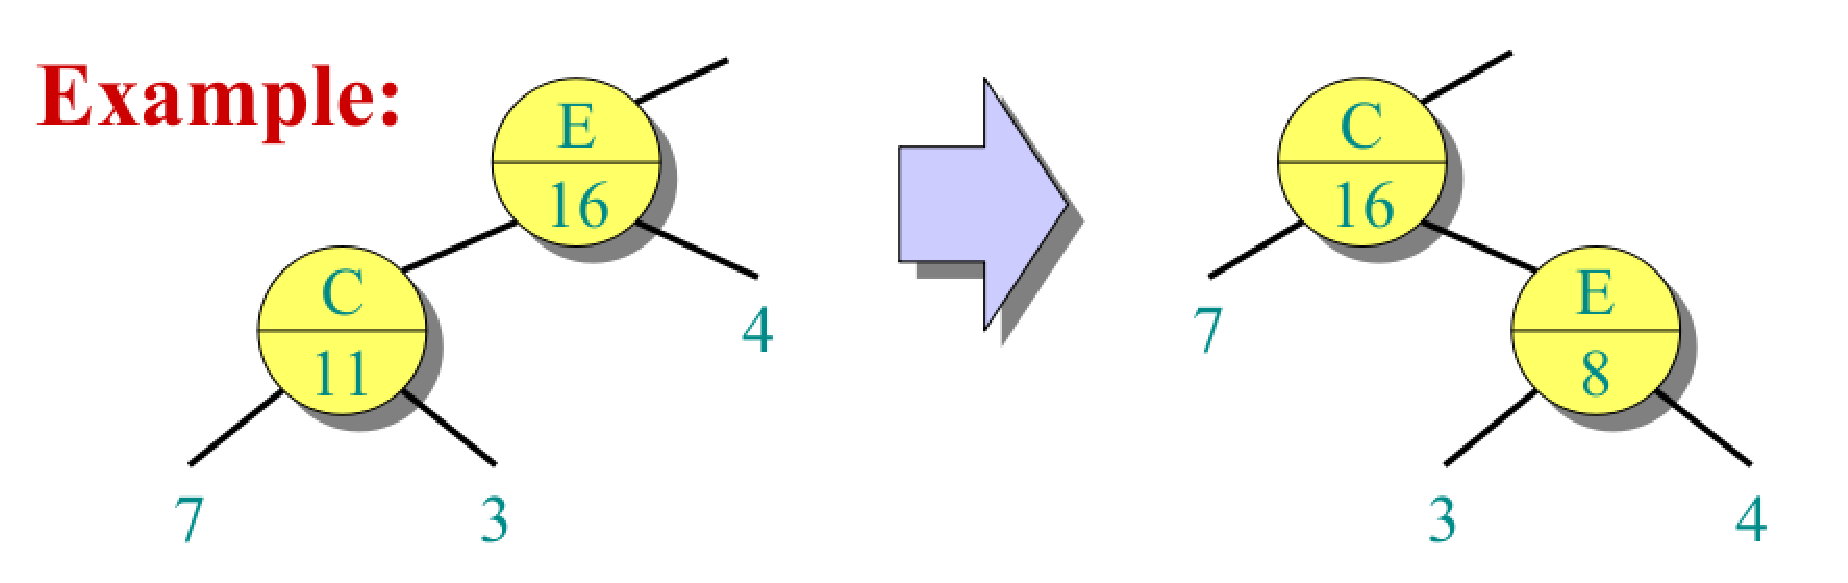
\includegraphics[width=5in]{lecture11/rotation.eps}
\end{center}

Таким образом, вставка продолжает выполняться за время $O(\lg n)$

То же можно сказать и об удалении.

\section{Методология расширения структур данных}

\begin{enumerate}
\item Выбрать подходящую СД (красно-чёрные деревья)
\item Определить дополнительную информацию, которая будет храниться в СД
  (размеры поддеревьев)
\item Проверить, что эта информация может поддерживаться при модифицирующих
  операциях (удаление, вставка в КЧ-деревьях, учитывая повороты)
\item Задать новые операции, которые решают изначально поставленные задачи на
  основе дополнительной информации (OS-Select, OS-Rank)
\end{enumerate}

Все эти шаги -- это набор рекомендаций, а не строгое пошаговое руководство к
действию. Обычно они выполняются в любом удобном порядке.

\section{Деревья отрезков}

Цель: поддерживать динамическое множество отрезков (например временных
промежутков).

\begin{center}
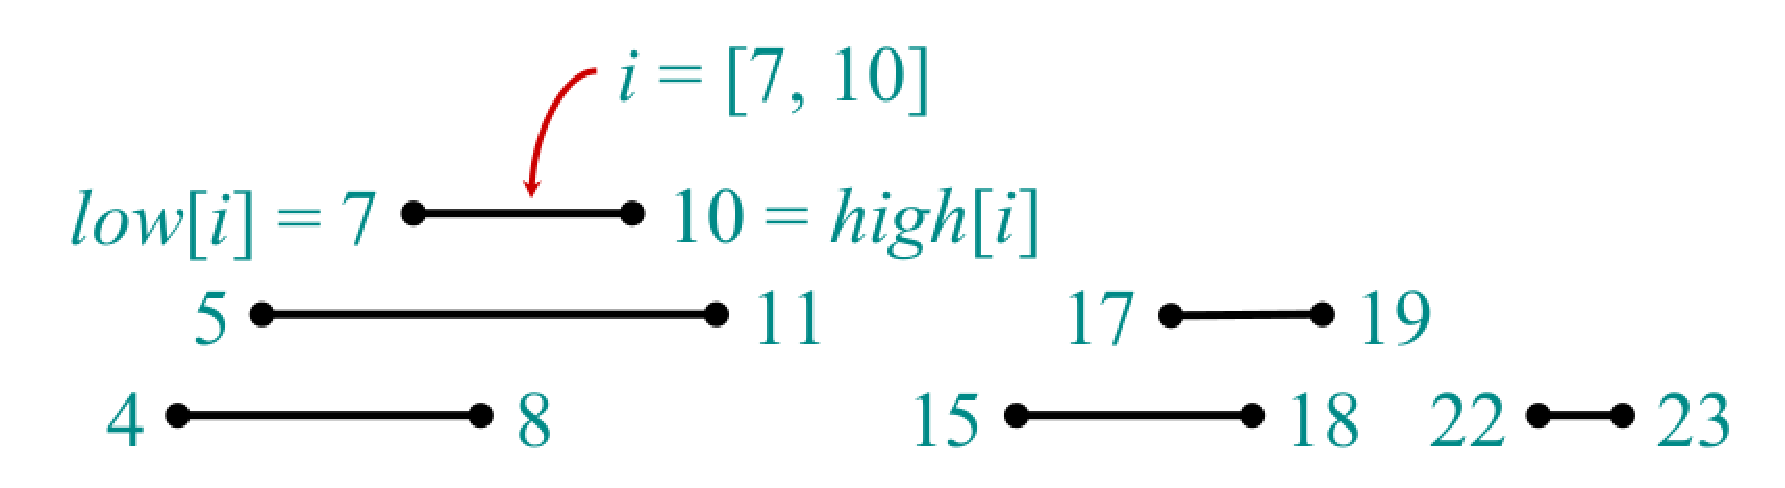
\includegraphics[width=5in]{lecture11/intervals.eps}
\end{center}

Задача: Для любого заданного отрезка $i$, найти отрезок, который перекрывается с
заданным и находится в нашем множестве (любой, если их несколько).

Следуем методологии:

\begin{enumerate}
\item Выбираем структуру данных: КЧ-деревья, в качестве ключа -- нижняя граница
  отрезка. Таким образом, центрированный обход дерева приводит к перечислению
  отрезков в порядке сортировки по их левым концам.
\item Дополнительная информация: будем хранить в каждом узле $x$ значение
  $max[x]$, которое представляет собой максимальное значение всех конечных точек
  отрезков, хранящихся в поддереве, корнем которого является $x$. Проще говоря:
  самую правую точку поддерева отрезков.
\item Поддержка информации: после вставки мы должны пересчитать значение $max$,
  это можно сделать с помощью формулы:

  $$
  max[x] = \max(high[int[x]], max[left[x]], max[right[x]])
  $$

  \begin{center}
    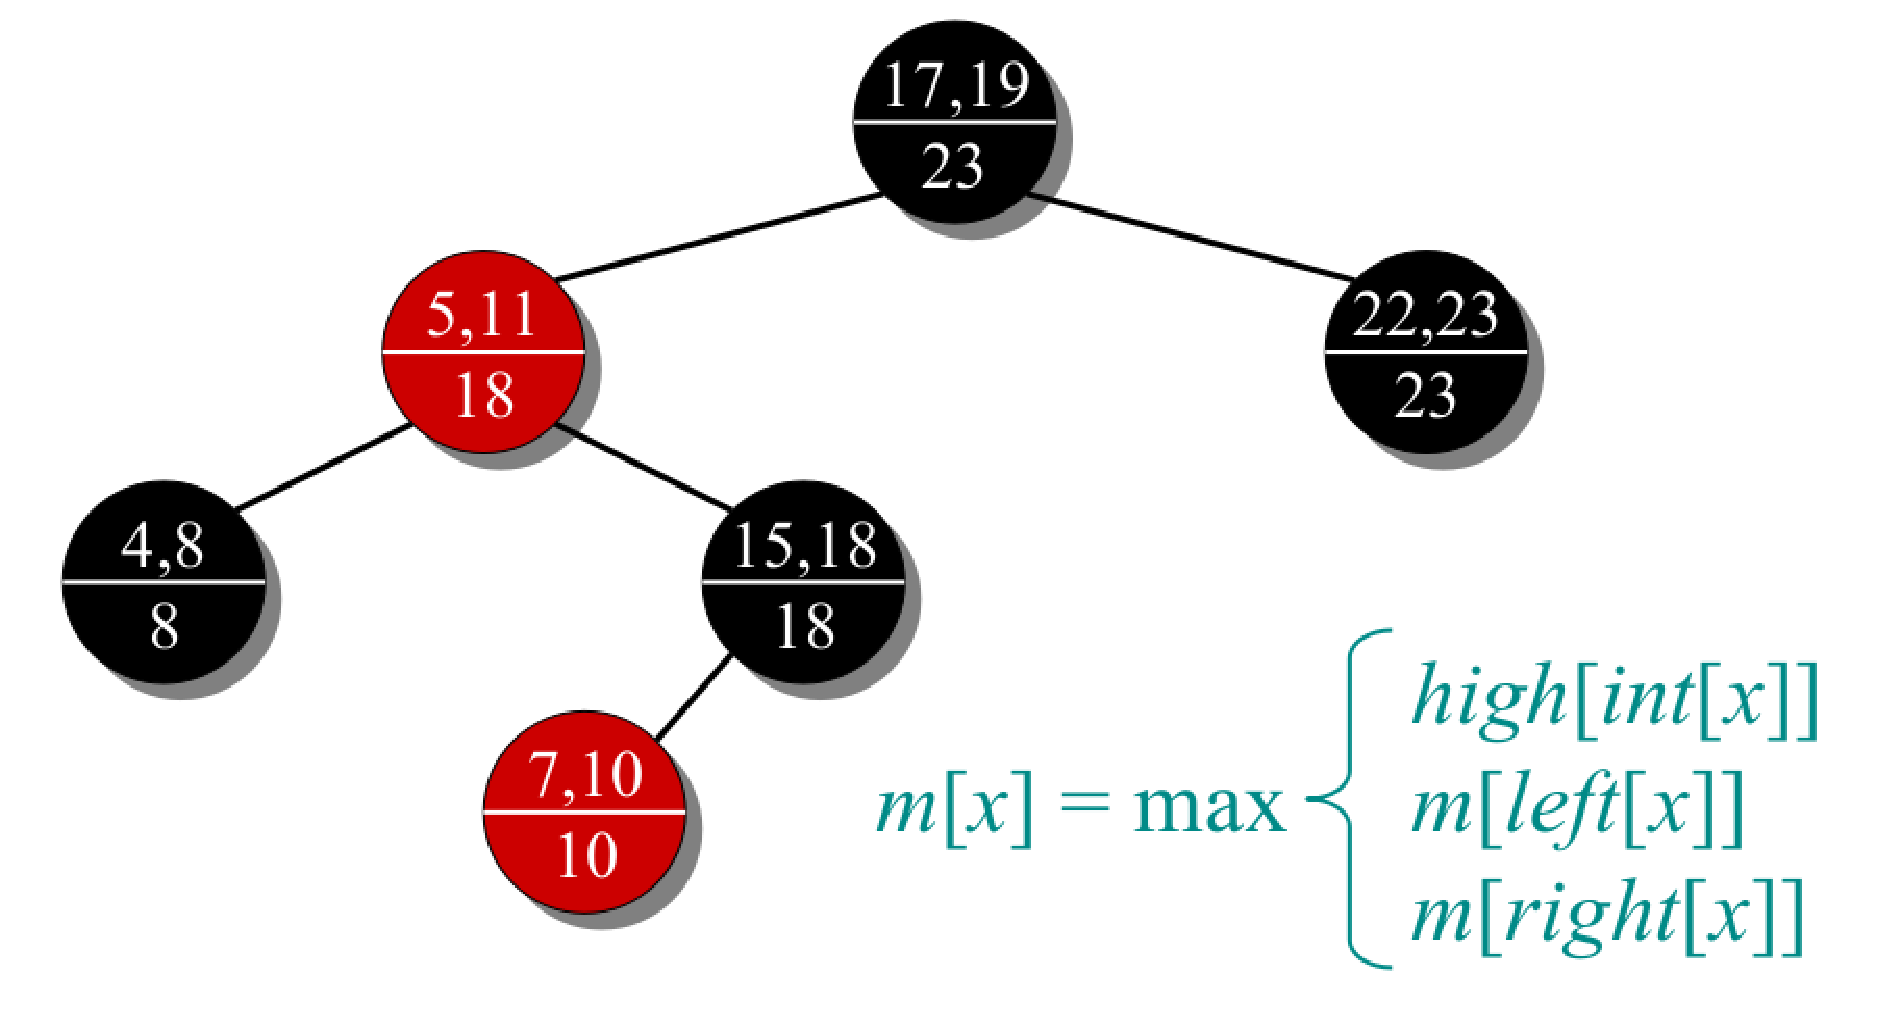
\includegraphics[width=5in]{lecture11/rb.eps}
  \end{center}
  
  Выполняем пересчёт $max$ по мере спуска от корня, в процессе поиска места в
  дереве, куда будет производится вставка. Затем нужно выполнить балансировку, в
  частности вращения. Во время вращений вычисление $max$ выполняется за
  константное время. Таким образом, операции вставки (аналогично и удаления)
  продолжают выполнятся за $O(\log n)$

  \begin{center}
    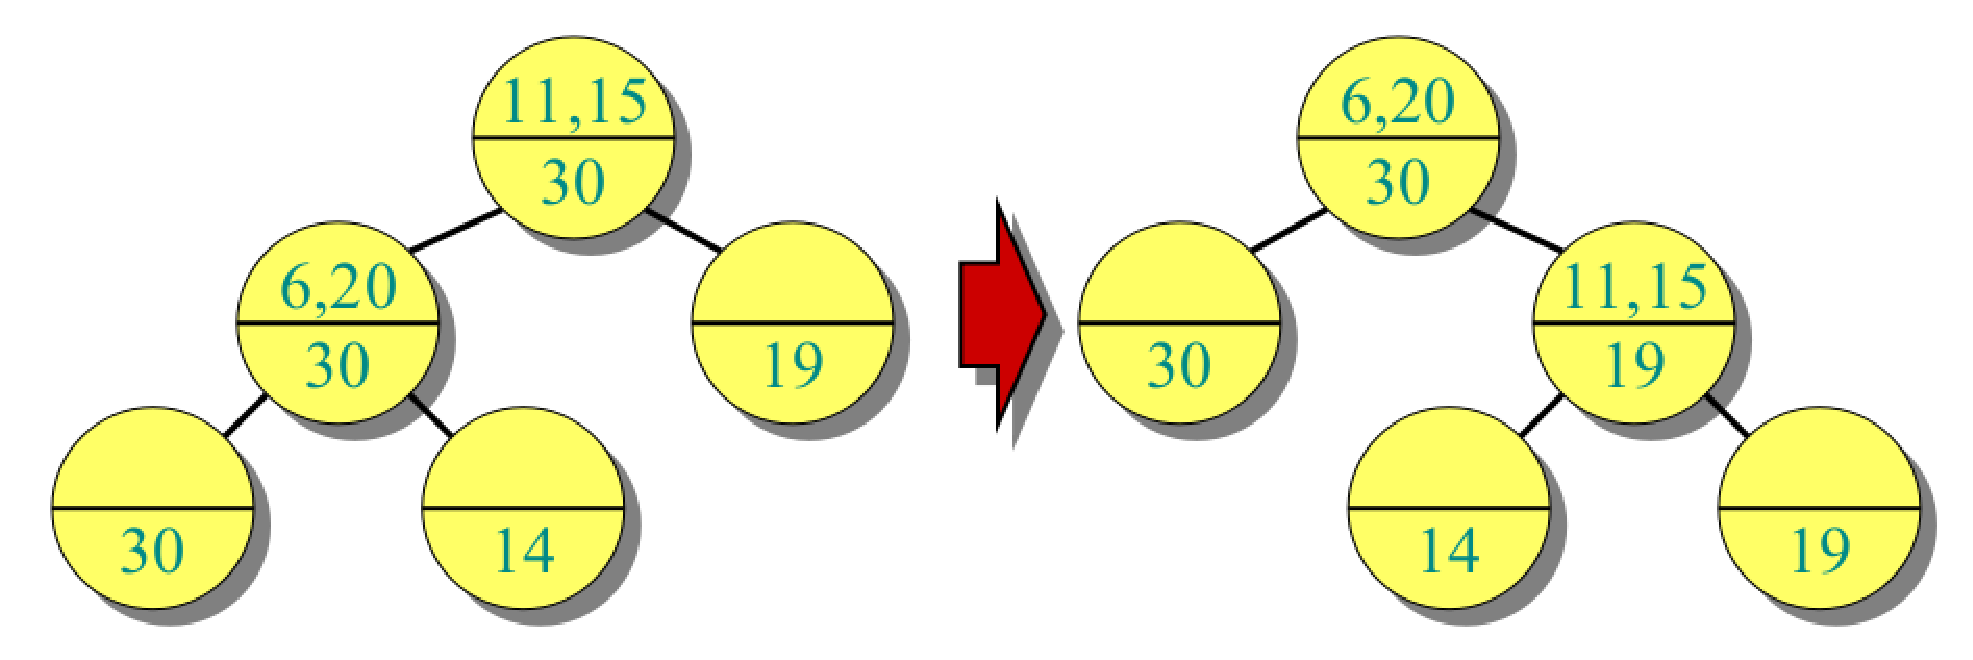
\includegraphics[width=5in]{lecture11/rotations-fixup.eps}
  \end{center}

  
\item Новые операции.
 
\begin{codebox}
\Procname{$\proc{Interval\_Search}(T, i)$}
\li $x \gets root[T]$
\li \While $x \neq NIL$ и $i$ не перекрывается с $int[x]$
\li \Do \If $left[x] \neq NIL$ и $ low[i] \leq max[left[x]]$
\li \Then $x \gets left[x]$
\li \Else $x \gets right[x]$
\End
\End
\li \Return $x$
\end{codebox}

\end{enumerate}

Пример поиска отрезка $[14, 16]$:

\begin{center}
  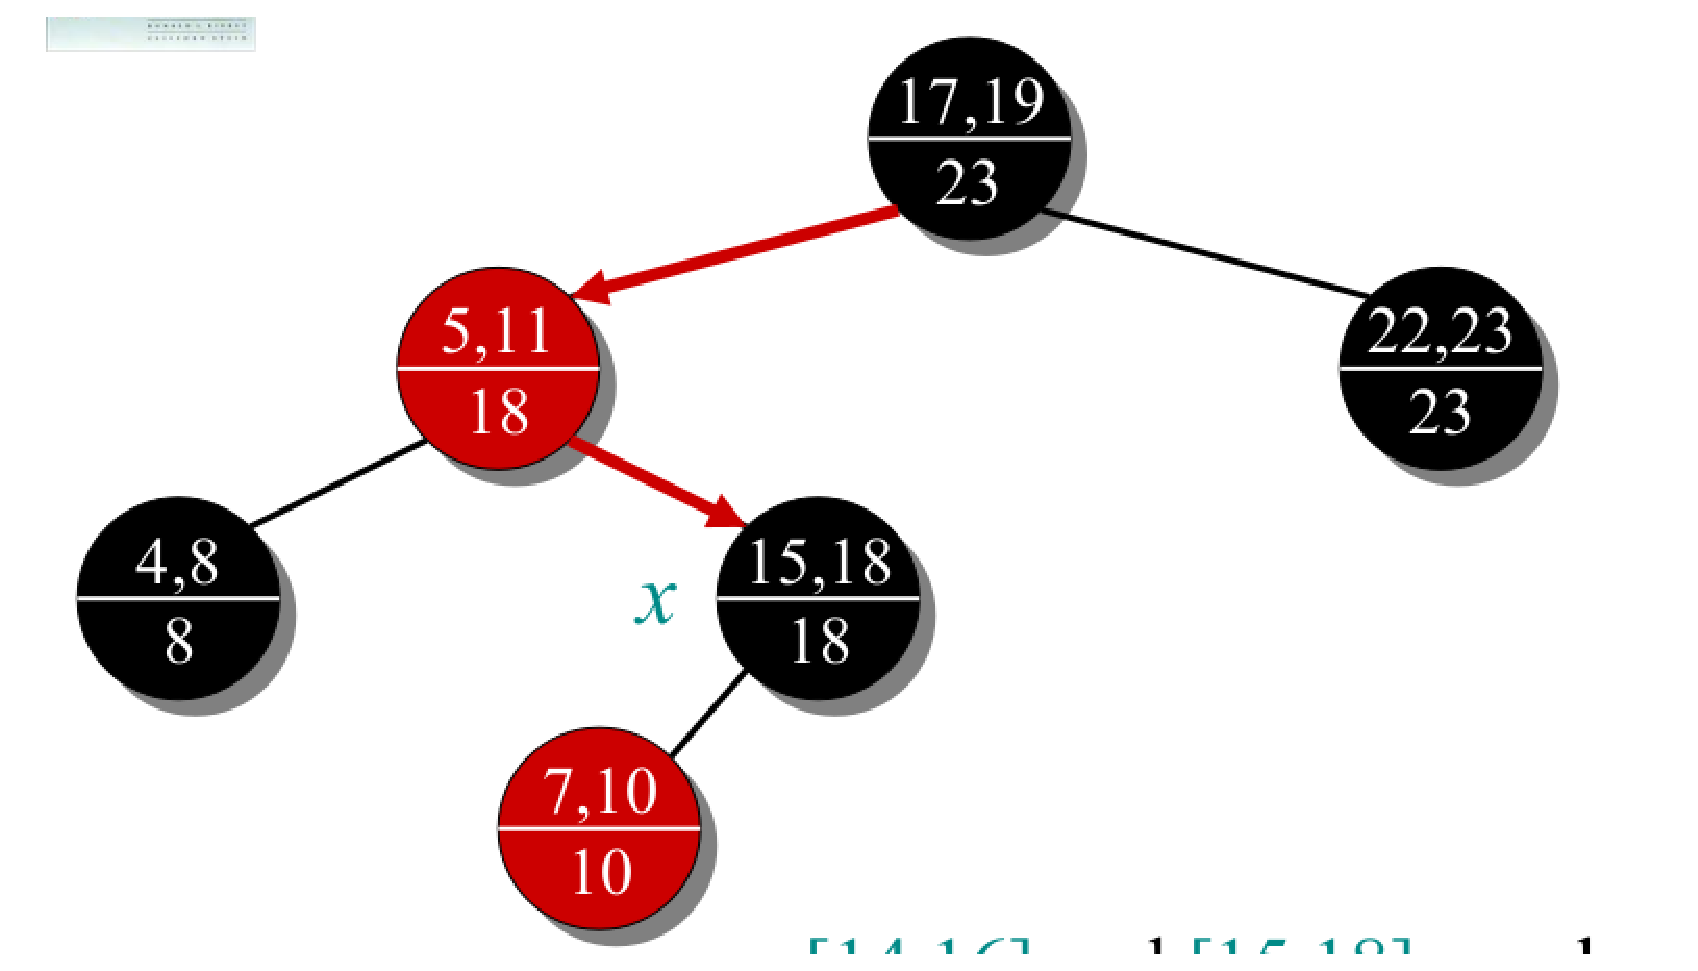
\includegraphics[width=5in]{lecture11/interval-search.eps}
\end{center}

\begin{itemize}
  
\item начинаем с корня дерева ($[17, 19]$)
\item проверяем не перекрывается ли текущий узел дерева (корень) с искомым
  отрезком (сравниваем $[14, 16]$ и $[17, 19]$ -- не перекрываются)
\item переходим к условию, т.е. сравниваем $low[i] = 14$ с $max[left[x]] =
  18$, меньше -- значит переходим к левому потомку ($[5, 11]$)
\item снова проверяем не перекрывается ли текущий узел дерева с искомым
  отрезком (сравниваем $[14, 16]$ и $[5, 11]$ -- не перекрываются)
\item снова переходим к условию, т.е. сравниваем $low[i] = 14$ с $max[left[x]] =
  8$, больше -- значит переходим к правому потомку ($[15, 18]$)
\item снова проверяем не перекрывается ли текущий узел дерева с искомым
  отрезком (сравниваем $[14, 16]$ и $[15, 18]$ -- перекрываются)
\item возвращаем $[15, 18]$
  
\end{itemize}

На примере $[12, 14]$ можно показать как работает алгоритм, когда дерево не
содержит перекрывающихся с заданным отрезков.

Анализ: $O(\lg n)$, т.к. каждый шаг мы делаем элементарные операции и
спускаемся вниз на один уровень, т.е. время выполнения пропорционально высоте
дерева.

Для поиска всех перекрывающихся отрезков можно применить такую технику:
найти, вывести, удалить, снова найти и т.д. После завершения поиска все
удалённые отрезки добавить вновь. Время выполнения такого алгоритма $O(k
\log n$, где $k$ -- количество выведенных отрезков. Такой алгоритм зависит от
вывода, т.е. от того сколько он выводит.

Лучший известный результат на сегодня: $O(k + \log n)$

\subsection{Доказательство корректности}

Идея: на каждом шаге мы выбираем куда идти: влево или вправо. Если нам удастся
показать, что мы всегда выбираем правильный путь, то нам удастся доказать
корректность. ``Правильный путь'' означает, что мы всегда выдадим
перекрывающийся интервал, если он есть.

Теорема: Пусть $L$ -- множество отрезков из левого поддерева узла $x$, т.е.
$$
L = \lbrace i' \in left[x] \rbrace
$$

$R$ -- множество отрезков из правого поддерева узла $x$, т.е.
$$
R = \lbrace i' \in right[x] \rbrace
$$

\begin{itemize}
  
\item если поиск идёт вправо, то
  $$
  \lbrace i' \in L \colon i' \text{ перекрывается с } i\rbrace = \emptyset
  $$
  
\item если поиск идёт влево, то
  \begin{align*}
  \lbrace i' \in L \colon i' \text{ перекрывается с } i\rbrace = \emptyset \\
  \Rightarrow
  \lbrace i' \in R \colon i' \text{ перекрывается с } i\rbrace = \emptyset
  \end{align*}

\end{itemize}

Другими словами: всегда безопасно выбирать только одного из детей узла дерева: мы
либо найдём то, что нужно, а если не найдём -- то значит ничего и не было.

Доказательство. Рассмотрим два случая:

\begin{enumerate}
\item Пусть поиск пошёл вправо.

  Такое возможно (см. псевдокод алгоритма) если $left[x] = NIL$, тогда поскольку
  левого поддерева нет вообще, выполняется $L = \emptyset$

  Иначе, чтобы поиск пошёл влево необходимо чтобы $low[i] > max[left[x]]$.
  Значение $max[left[x]]$ соответствует самой правой точке некого отрезка $j$ из
  множества $L$. Поскольку эта точка \emph{самая правая}, то никакой другой
  отрезок из $L$ не может иметь свою правую точку ещё правее чем $high[j]$.

  \begin{center}
    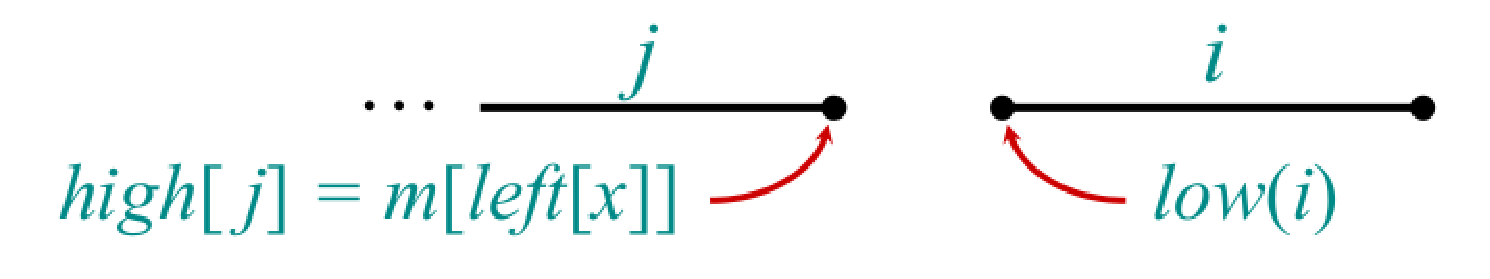
\includegraphics[width=5in]{lecture11/correctness1.eps}
  \end{center}
  
  Таким образом,
  $$
  \lbrace i' \in L \colon i' \text{ перекрывается с } i\rbrace = \emptyset
  $$

\item Пусть поиск пошёл влево.

  Также по условию теоремы мы предполагаем, что
  $$
  \lbrace i' \in L \colon i' \text{ перекрывается с } i\rbrace = \emptyset
  $$

  Согласно псевдокоду алгоритма: $$ low[i] \leq m[left[x]] = high[j] $$ для
  некоего отрезка $j$ из $L$.

  Поскольку $j \in L$, то согласно предпосылке теоремы $j$ не пересекается с
  $i$ и как следствие получаем, что $high[i] < low[j]$ (т.к. существуют всего
  три варианта взаимного расположения отрезков, они либо перескаются, либо
  первый слева от второго, либо первый справа от второго).

  Теперь, используя свойство двоичных деревьев поиска и учитывая, что в качестве
  ключа мы используем левую точку отреза, отметим, что для всех $i' \in R$
  выполняется $low[j] \leq low[i']$

  В таком случае:
  $$
  \lbrace i' \in R \colon i' \text{ перекрывается с } i\rbrace = \emptyset
  $$

  \begin{center}
    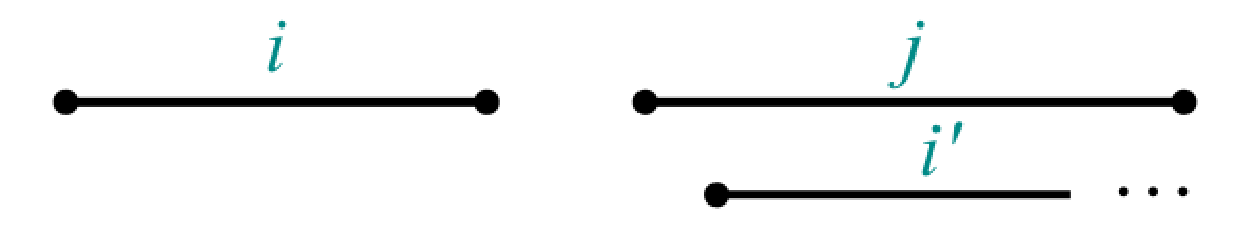
\includegraphics[width=5in]{lecture11/correctness2.eps}
  \end{center}

  Что и требовалось доказать.
  
\end{enumerate}
  
\end{document}

